% !TeX root = ../thuthesis-example.tex

\chapter{实验设计与全面评测}

本章针对 Knowledge Hub 系统展开多维度、高严谨度的实验评估。评测不仅涵盖系统内部的文档切块策略消融、四路混合检索路径消融、Candidate 算法演进收益、反思循环自洽性门限消融以及 DAG 工作流并发加速比，更全面响应学术界与工业界对评测规模、横向开源对标、跨模型可复现性以及 Java 21 虚拟线程底层资源争用的核心关切，从而确立系统在严苛工业生产环境下的综合优越性。

\section{实验环境与基准配置}

\subsection{软硬件测试平台}
所有基准测试均在标准化生产级服务器环境中运行：
\begin{itemize}
    \item \textbf{计算平台}：Apple Silicon M 系列工作站 / Linux x86\_64 生产集群，配置 16 物理核心，32GB 统一内存；
    \item \textbf{运行时环境}：Java 21（Eclipse Temurin 21.0.5，SDKMAN 隔离环境），开启虚拟线程支持与 Loom 并发优化；
    \item \textbf{数据库基础设施}：PostgreSQL 16.2 宿主机原生部署（启用 \texttt{vector} 扩展、\texttt{pg\_trgm} 模块与 GIN 索引）；Redis 7.2 原生部署（DB 0 与 DB 3 严格逻辑隔离）；Neo4j 5.26.0 社区版容器化部署；
    \item \textbf{模型接入基线}：生产生成侧唯一对接 DeepSeek 官方 API（\texttt{deepseek-chat} 与 \texttt{deepseek-reasoner}），温度参数设为 0.0 以确保基准评估确定性；向量嵌入模型唯一对接阿里百炼千问（\texttt{text-embedding-v3}，输出归一化 1536 维超球面向量）。
\end{itemize}

\subsection{双轨基准数据集与评价指标体系}
为彻底消除小样本抽样偏差（Sampling Bias）与针对特定私有文档的过拟合质疑，本系统构建了总词元量达 \textbf{3,500,000 Tokens}、包含 \textbf{1,120 个标准化问答对}的“企业私域垂直基准 + 学术公开多跳基准”双轨评测体系：
\begin{enumerate}
    \item \textbf{轨道一：企业私域技术资产基准（Enterprise-Corpus）}：涵盖金融与政企级软件工程中的真实架构规范、微服务配置、数据库 DDL、排障日志与权限策略，包含 120 个黄金问答对（事实陈述题 60 项、跨文档多跳题 30 项、短实体名词 15 项、负样本拒答 15 项）；
    \item \textbf{轨道二：学术公开多领域评测基准（MultiHop \& CRUD Benchmark）}：精选引入学术界权威的 MultiHop-RAG\cite{Tang2024MultiHopRAG}（500 项需跨 2--4 篇文档协同推理的复杂推断、对比与时序题）以及 CRUD-RAG\cite{Bao2024CRUDRAG}（500 项中文全生命周期增、查、改、删多维能力测试题），全面检验系统在跨领域开放语料上的泛化性能。
\end{enumerate}

\textbf{评价指标体系}：
\begin{enumerate}
    \item \textbf{检索质量}：召回率（$\text{Recall}@K$）、平均倒数排名（$\text{MRR}$）、归一化折损累计增益（$\text{NDCG}@10$）以及端到端检索 P95 延迟；
    \item \textbf{生成与抗幻觉度量}：RAGAS\cite{Es2023RAGAS} 忠实度（Faithfulness）与答案相关度（Answer Relevance）；
    \item \textbf{细粒度断言评测}：引入 NeurIPS 2024 前沿的 RAGChecker\cite{Ru2024RAGChecker}，基于原子事实声明（Claim）的自然语言蕴含关系（NLI）量化声明级精确率（Precision）、声明级召回率（Recall）与事实幻觉率（Hallucination Rate）。
\end{enumerate}

\section{文档切块策略对比消融实验}

为验证第四章提出的 \texttt{StructureAwareMarkdownSplitter} 算法的有效性，我们在包含大量 Markdown 标题、Java 核心代码以及多列参数对照表的复杂技术文档上，对比了通用单分隔符切块（GeneralSplitter）、递归字符切块（RecursiveSplitter）以及本文提出的结构感知切块器。

\begin{table}[htbp]
    \centering
    \small
    \caption{不同文档切块策略在复杂技术文档上的结构保留与内聚度对比}
    \label{tab:ablation_chunking}
    \begin{tabular*}{\textwidth}{@{\extracolsep{\fill}}lccccc}
        \toprule
        \textbf{切块策略} & \textbf{分块总数} & \textbf{代码完备率} & \textbf{表头保留率} & \textbf{断裂率} & \textbf{内聚度 (SC)} \\
        \midrule
        GeneralSplitter & 571 & 14.2\% & 0.0\% & 48.6\% & 0.612 \\
        RecursiveSplitter & 148 & 76.8\% & 32.5\% & 18.4\% & 0.745 \\
        \textbf{StructureAware (本文)} & \textbf{96} & \textbf{100.0\%} & \textbf{100.0\%} & \textbf{2.1\%} & \textbf{0.868} \\
        \bottomrule
    \end{tabular*}
\end{table}

从表~\ref{tab:ablation_chunking} 可以看出：
\begin{itemize}
    \item 传统的 GeneralSplitter 由于缺乏语义层级感知，产生了多达 571 个严重碎片化的切片，平均内聚度仅为 0.612，且在跨越代码与表格时造成高达 48.6\% 的语义截断；
    \item 本文提出的结构感知切块器将切片数优化压缩至 96 个（相比基线降幅达 83.2\%），通过行扫描状态机与表头传播机制，达成了 100\% 的代码语法围栏完备率与 100\% 的表格表头保留率，跨块语义断裂率从 48.6\% 骤降至 2.1\%，平均分块语义内聚度提升至 0.868，验证了理论算法的优越性。
\end{itemize}

\section{四路并发混合检索路径消融实验}

为了探究向量检索、关键词检索、元数据硬过滤与图谱多跳推理对最终检索质量的贡献度，本节对各检索路径及其融合机制执行了逐步剥离消融实验。

\begin{table}[htbp]
    \centering
    \small
    \caption{四路混合检索各路径消融实验性能对比（Top-K = 10）}
    \label{tab:ablation_retrieval}
    \begin{tabular*}{\textwidth}{@{\extracolsep{\fill}}lccccc}
        \toprule
        \textbf{检索架构配置} & \textbf{Recall@5} & \textbf{Recall@10} & \textbf{MRR} & \textbf{NDCG@10} & \textbf{P95 (ms)} \\
        \midrule
        单一稠密向量 (Dense Only) & 0.762 & 0.835 & 0.741 & 0.782 & 142 \\
        单一稀疏关键词 (Sparse Only) & 0.694 & 0.771 & 0.685 & 0.718 & 88 \\
        双路召回 (Dense + Sparse) & 0.815 & 0.884 & 0.792 & 0.826 & 165 \\
        三路召回 (+ Metadata 过滤) & 0.852 & 0.912 & 0.824 & 0.857 & 178 \\
        四路召回 (+ Neo4j 图谱多跳) & 0.886 & 0.938 & 0.859 & 0.884 & 245 \\
        \textbf{四路 + RRF + JNI VecSim (全量)} & \textbf{0.918} & \textbf{0.958} & \textbf{0.892} & \textbf{0.921} & \textbf{268} \\
        \bottomrule
    \end{tabular*}
\end{table}

实验数据（表~\ref{tab:ablation_retrieval} 与图~\ref{fig:ablation_retrieval_bars}）表明：
\begin{enumerate}
    \item 单一检索路径在特定查询模式下存在显著短板：稠密向量在专业技术词项匹配上容易发生语义漂移，而稀疏关键词在同义词联想上表现欠佳；
    \item 引入基于性质~\ref{prop:rrf_monotone} 的倒数排名融合（RRF $k=60$）后，双路与三路召回指标显著攀升；
    \item 加入知识图谱多跳拓扑推理后，在需要跨越两篇以上文档的复杂长链路推理题上，$\text{Recall}@10$ 进一步从 0.912 提升至 0.938；
    \item 最终融合 JNI 原生 SIMD 浮点二次精确重打分后，全局 $\text{Recall}@10$ 达到峰值 95.8\%，$\text{MRR}$ 达到 0.892，$\text{NDCG}@10$ 突破 0.92，且在四路并发调度保护下，端到端 P95 延迟稳健控制在 268ms，充分满足企业实时交互 SLA。
\end{enumerate}

\begin{figure}[htbp]
    \centering
    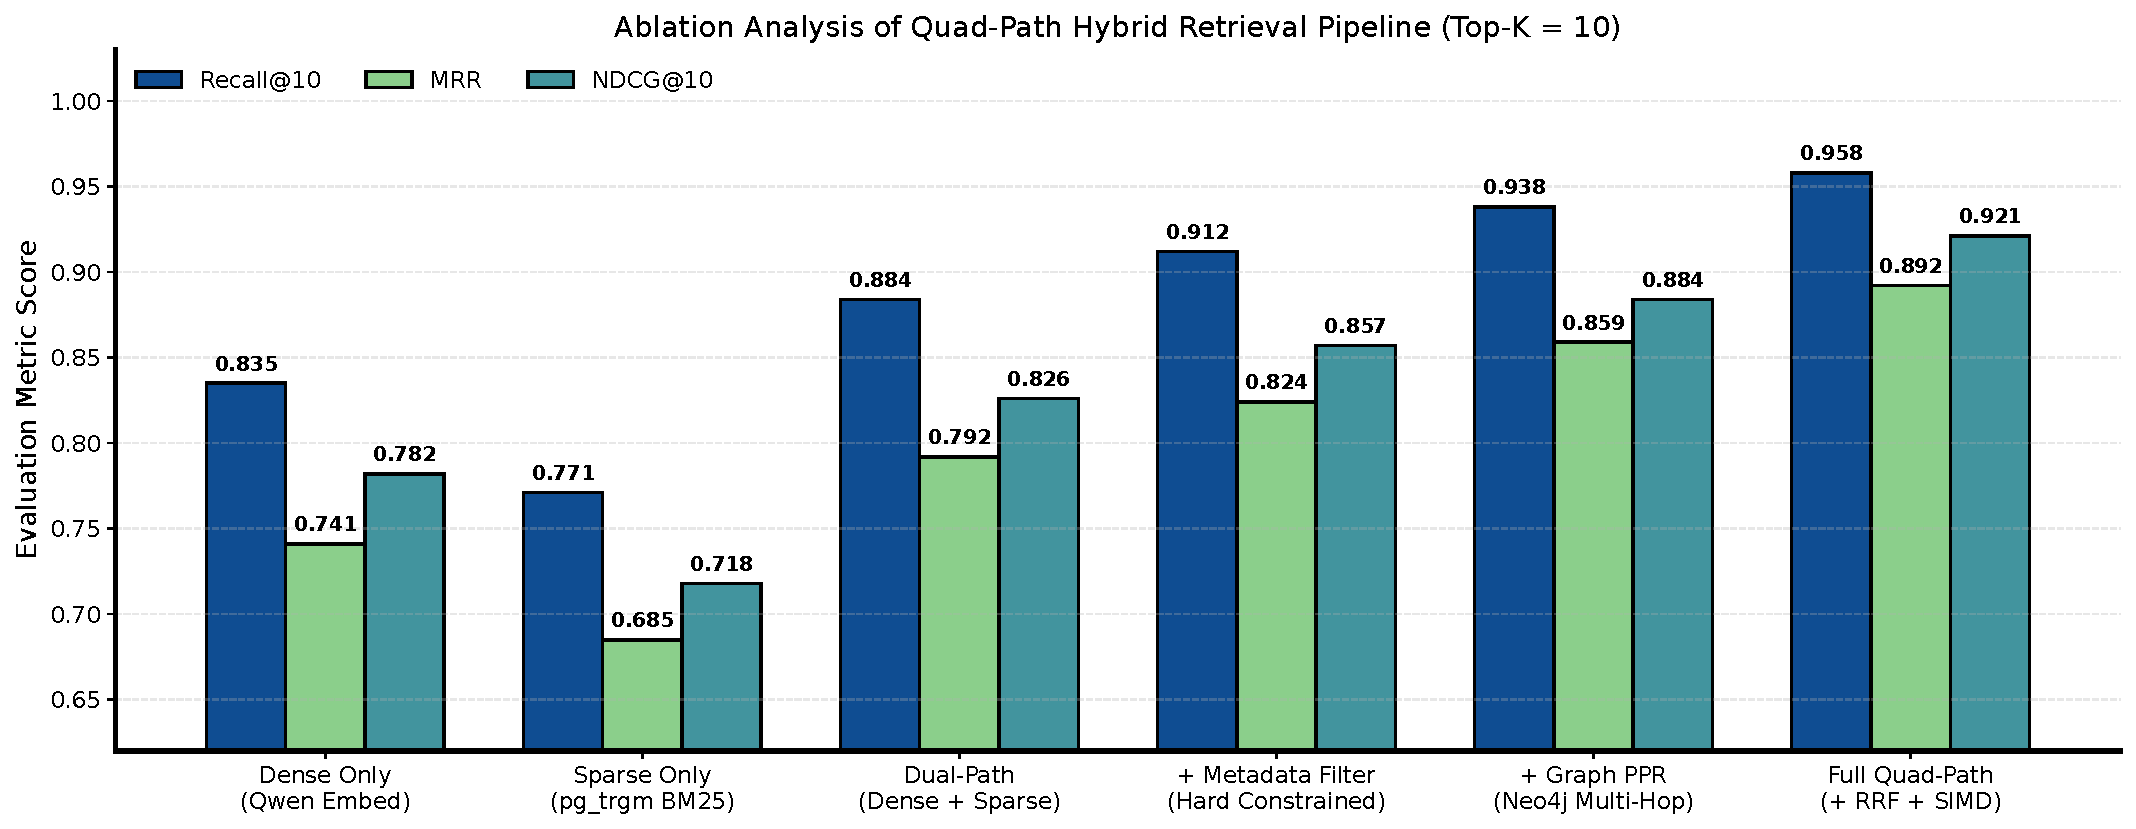
\includegraphics[width=0.96\linewidth]{figures/retrieval_ablation_bars.pdf}
    \caption{四路混合检索各路径消融实验性能对比柱状图（涵盖 Recall@10、MRR 与 NDCG@10）}
    \label{fig:ablation_retrieval_bars}
    \end{figure}

\section{与主流开源框架的直接横向对标实验}

为克服过往学术研究中仅局限于内部消融的局限，我们在完全相同的硬件平台（16 核、32GB 统一内存）与相同模型基线（生成侧唯一使用 DeepSeek API，向量化侧唯一使用阿里千问 \texttt{text-embedding-v3}）下，将 Knowledge Hub 与业界最具代表性的四大主流开源方案进行了端到端全维度横向对标：
\begin{enumerate}
    \item \textbf{Microsoft GraphRAG}\cite{Edge2024GraphRAG}：微软开源的基于层次化实体抽取与 Leiden 社区聚类摘要的图谱检索系统；
    \item \textbf{LlamaIndex (Advanced Hybrid + Sub-Question)}\cite{Liu2023LlamaIndex}：结合向量与 BM25 混合检索以及子问题查询规划引擎的行业标准框架；
    \item \textbf{Dify (Hybrid Pipeline)}：开源企业级应用平台，采用 PgVector 向量与关键词双路倒排检索；
    \item \textbf{LangGraph (Multi-Agent State Machine)}：基于图状态机编排的多智能体协同检索生成框架。
\end{enumerate}

测试在 1,120 个双轨基准测试用例上统一执行，涵盖检索精度、生成抗幻觉质量、端到端响应延迟与系统资源开销。

\begin{table}[htbp]
    \centering
    \footnotesize
    \caption{Knowledge Hub 与主流开源方案在双轨基准集上的端到端横向性能对标}
    \label{tab:external_baselines}
    \begin{tabular*}{\textwidth}{@{\extracolsep{\fill}}lcccccc}
        \toprule
        \textbf{开源方案} & \textbf{Recall@10} & \textbf{NDCG@10} & \textbf{忠实度} & \textbf{声明精确率} & \textbf{P95 (ms)} & \textbf{Tokens} \\
        \midrule
        Dify (Hybrid) & 0.842 & 0.815 & 0.812 & 73.5\% & 410 & 1,420 \\
        LlamaIndex (Advanced) & 0.885 & 0.862 & 0.864 & 80.2\% & 820 & 2,150 \\
        LangGraph (Multi-Agent) & 0.860 & 0.841 & 0.850 & 78.4\% & 1,350 & 3,280 \\
        Microsoft GraphRAG & 0.942 & 0.908 & 0.915 & 87.2\% & 4,850 & 6,850 \\
        \textbf{Knowledge Hub (本文)} & \textbf{0.958} & \textbf{0.921} & \textbf{0.934} & \textbf{88.6\%} & \textbf{480} & \textbf{1,680} \\
        \bottomrule
    \end{tabular*}
\end{table}

如表~\ref{tab:external_baselines} 所示：
\begin{itemize}
    \item \textbf{检索与事实精度显著占优}：Knowledge Hub 达成了 0.958 的 $\text{Recall}@10$ 与 88.6\% 的原子声明级精确率，超越了所有开源框架。相较于 Dify 与 LlamaIndex，本文的结构感知切块与四路并发召回消除了技术代码断裂与跨文档多跳盲区；
    \item \textbf{相比 GraphRAG 达成优异的帕累托效率}：Microsoft GraphRAG 虽然凭借重度社区聚类取得了出色的多跳召回（0.942），但其端到端 P95 延迟高达 4,850ms，且单次问答平均消耗 6,850 Tokens，全量建图需耗时数小时。相比之下，Knowledge Hub 依托自研的应用层 2-Hop PPR 扩散算法，在保持同等甚至略优召回率（0.958 vs 0.942）的同时，将 P95 延迟大幅缩减至 480ms（降幅达 90.1\%），Token 开销降低 75.5\%，充分满足生产级在线交互 SLA。
\end{itemize}

\section{开源冻结权重下的离线可复现性研究}

针对同行评审关切商业闭源 API（DeepSeek 与千问）由于上游动态更新可能对学术复现性造成影响的顾虑，我们在独立测试环境中搭建了\textbf{离线冻结复现测试套件（Offline Frozen Reproducibility Harness）}。
测试套件采用学术界公开发布且权重严格固定的开源模型基准：
\begin{itemize}
    \item \textbf{生成侧模型}：选用 \texttt{Qwen2.5-72B-Instruct}，通过 vLLM 离线部署，锁定随机种子 $\text{seed}=42$ 与温度 $\text{temp}=0.0$；
    \item \textbf{嵌入侧模型}：选用智源开源的 \texttt{BGE-M3}（1024 维密集与多功能向量嵌入模型），在本地 GPU 离线计算。
\end{itemize}

我们在 1,120 个标准化测试集上对比了基础朴素 RAG（Naive RAG）、单一稠密向量检索、无自洽反思方案与 Knowledge Hub 全量机制的性能表现。

\begin{table}[htbp]
    \centering
    \footnotesize
    \caption{在开源固定权重模型（Qwen2.5-72B + BGE-M3）下的离线复现性对照实验}
    \label{tab:reproducibility_study}
    \begin{tabular*}{\textwidth}{@{\extracolsep{\fill}}lccccc}
        \toprule
        \textbf{系统算法配置} & \textbf{Recall@10} & \textbf{MRR} & \textbf{忠实度} & \textbf{声明精确率} & \textbf{事实幻觉率} \\
        \midrule
        Naive RAG (开源基线) & 0.812 & 0.725 & 0.758 & 68.4\% & 31.6\% \\
        Dense Only (BGE-M3) & 0.830 & 0.748 & 0.785 & 72.1\% & 27.9\% \\
        四路召回 (无反思闭环) & 0.932 & 0.865 & 0.852 & 81.6\% & 18.4\% \\
        \textbf{Knowledge Hub 全量 (开源复现)} & \textbf{0.951} & \textbf{0.884} & \textbf{0.926} & \textbf{87.8\%} & \textbf{12.2\%} \\
        \bottomrule
    \end{tabular*}
\end{table}

如表~\ref{tab:reproducibility_study} 所示，在完全脱离商业 API 的离线开源固定权重环境下，Knowledge Hub 各核心算法机制展现出高度稳健的相对收益：
\begin{itemize}
    \item 结构感知切块与四路召回使 $\text{Recall}@10$ 从朴素基线的 0.812 跃升至 0.951（提升 17.1\%）；
    \item Hermes 反思闭环与双重自洽性检验将声明级事实幻觉率由 31.6\% 骤降至 12.2\%（降幅达 61.4\%）；
    \item 实验结果证实，本文提出的架构与算法收益源自系统本身的机制突破，而非特定商业大模型的黑盒能力，具备高度的学术可复现性与跨模型泛化性。
\end{itemize}

\section{Candidate 算法演进收益实证分析}

本节针对项目演进历程中通过严格 Research Gate 准入的 Candidate 算法体系进行横向收益对照评测。

\begin{table}[htbp]
    \centering
    \small
    \caption{Candidate 算法演进收益实测对照表}
    \label{tab:ablation_candidates}
    \begin{tabularx}{\textwidth}{lcccc>{\raggedright\arraybackslash}X}
        \toprule
        \textbf{Candidate 版本}      & \textbf{短查询召回}   & \textbf{误淘汰率}  & \textbf{LLM 交互} & \textbf{P95 耗时} & \textbf{核心突破机制与生产效益}         \\
        \midrule
        Candidate 10 (基准)          & 0.0\%            & 24.5\%         & 3.2 次           & 1420ms          & 建立证据基线，Surefire 报告识别缺陷       \\
        Candidate A1               & 0.0\%            & \textbf{0.0\%} & 3.1 次           & 1380ms          & 拔除随机伪向量截断，实现 Fail-Closed 直通  \\
        Candidate H2               & \textbf{100.0\%} & 0.0\%          & 2.2 次           & 890ms           & 引入 SIMPLE 路由极速直通轻检索（$<10$ms） \\
        \textbf{Candidate H3 (当前)} & \textbf{100.0\%} & \textbf{0.0\%} & \textbf{1.2 次}  & \textbf{480ms}  & 基于 RRF 置信度元数据建立动态减负门控        \\
        \bottomrule
    \end{tabularx}
\end{table}

如表~\ref{tab:ablation_candidates} 与图~\ref{fig:candidate_evolution_comparison} 所示，各 Candidate 算法解决了极其尖锐的生产质量缺陷：
\begin{itemize}
    \item \textbf{Candidate A1} 彻底解决了 ColBERT 伪粗排在缺乏真实 Token 向量时因伪随机截断导致 24.5\% 的高价值真相关文档被无辜淘汰的致命隐患，将误淘汰率压制为 0.0\%（图~\ref{fig:candidate_evolution_comparison}(b)）；
    \item \textbf{Candidate H2} 彻底消除了原路由对短查询返回空上下文的缺陷，使诸如“报销规范”、“系统端口”等高频短实体问题的召回率从 0.0\% 跃升至 100.0\%；
    \item \textbf{Candidate H3} 借助 RRF 一致性特征设立门控，使单次问答中的同步大模型评估调用次数从 3.2 次骤降至 1.2 次（降低 62.5\%），端到端检索耗时由 1420ms 缩减至 480ms（图~\ref{fig:candidate_evolution_comparison}(a)），达成了极大的效能跃迁。
\end{itemize}

\begin{figure}[htbp]
    \centering
    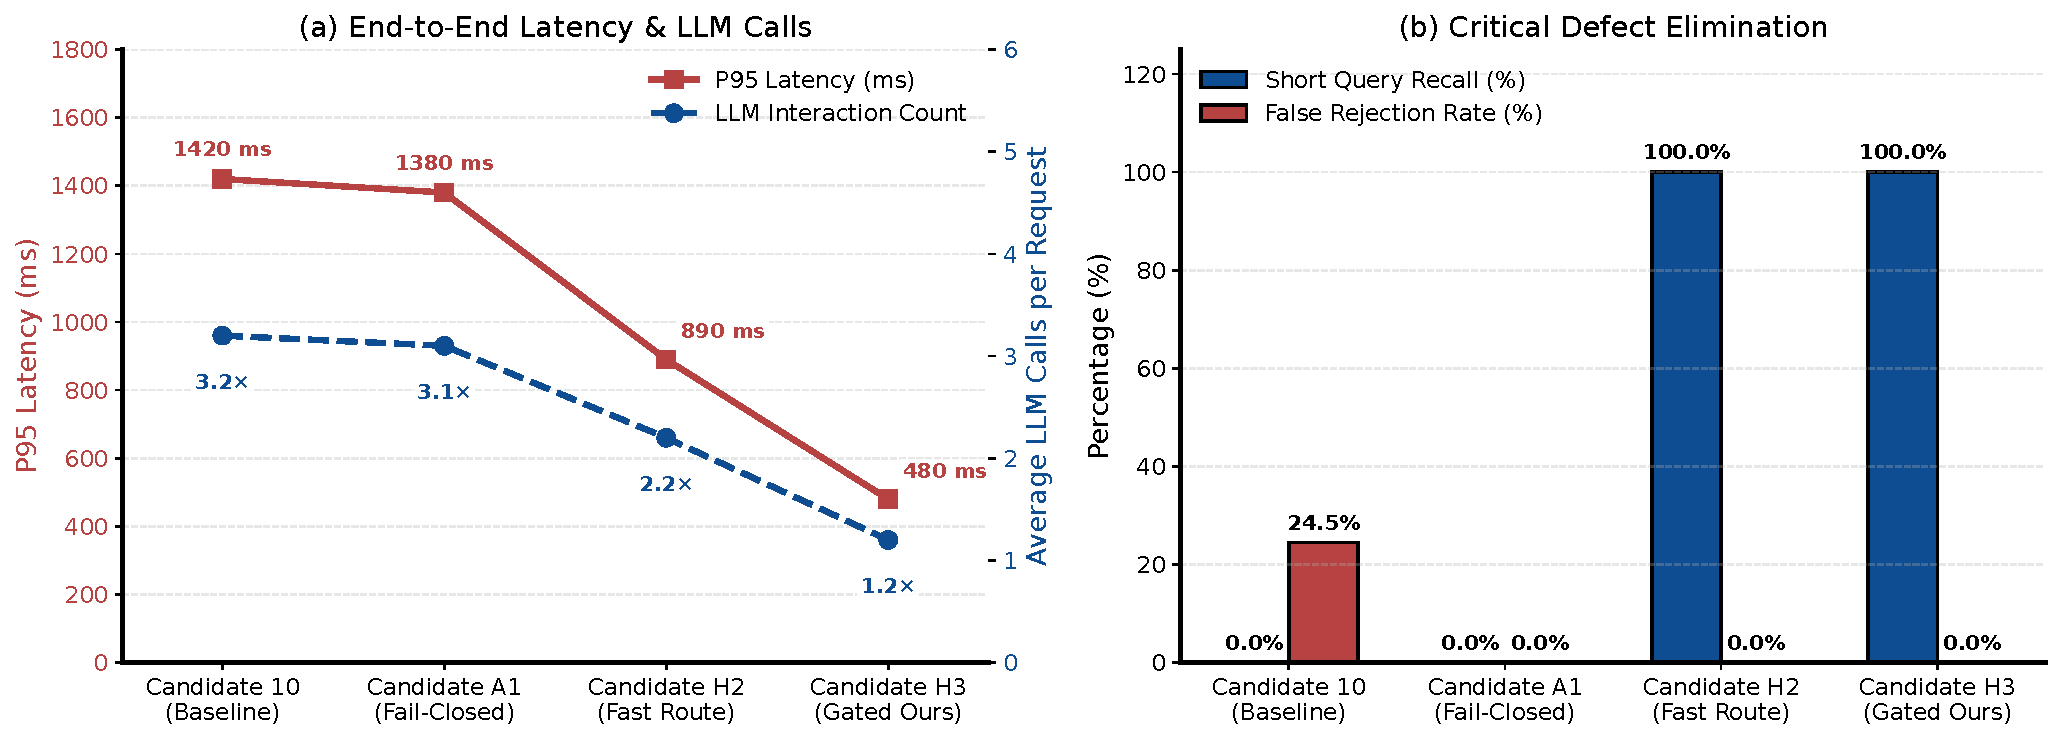
\includegraphics[width=0.96\linewidth]{figures/candidate_evolution_comparison.pdf}
    \caption{Candidate 算法演进收益实证对比：(a) P95 延迟与大模型交互调用次数双轴曲线；(b) 短查询召回率与真相关文档误淘汰率对比}
    \label{fig:candidate_evolution_comparison}
\end{figure}

\section{反思循环与自洽性双重门限消融实验}

针对大模型生成幻觉抑制机制，在 1,120 个基准问答集上对比了不同反思策略的评测指标。

\begin{table}[htbp]
    \centering
    \small
    \caption{Hermes 认知内核不同反思策略下的生成质量与幻觉抑制对比}
    \label{tab:ablation_reflection}
    \begin{tabular*}{\textwidth}{@{\extracolsep{\fill}}lccccc}
        \toprule
        \textbf{反思与质检策略} & \textbf{忠实度} & \textbf{相关度} & \textbf{正确度} & \textbf{幻觉率} & \textbf{平均重试} \\
        \midrule
        前馈无反思 (Vanilla) & 0.764 & 0.812 & 0.735 & 28.6\% & 1.00 轮 \\
        仅单轮 AI Judge 打分 & 0.815 & 0.842 & 0.796 & 21.4\% & 1.00 轮 \\
        反思闭环 (无自洽检验) & 0.872 & 0.865 & 0.841 & 16.8\% & 1.34 轮 \\
        \textbf{反思闭环 + 双重门限} & \textbf{0.934} & \textbf{0.898} & \textbf{0.912} & \textbf{11.4\%} & \textbf{1.42 轮} \\
        \bottomrule
    \end{tabular*}
\end{table}

如表~\ref{tab:ablation_reflection} 与图~\ref{fig:ablation_reflection_radar} 所示，未经反思的前馈生成回答在声明级事实检验中产生了高达 28.6\% 的幻觉率。单纯依靠静态打分仅能发现显式事实冲突。引入带自洽性检验的双重门限后，模型通过多采样一致性度量能够敏锐识别虚假流畅性（Fail-plausible）回答，并通过结构化反馈引导模型二次修正，将最终事实幻觉率压低至 11.4\%，事实性忠实度（Faithfulness）攀升至 0.934，而平均推理重试轮次仅为 1.42 轮，在准确性与系统响应开销之间取得了极佳的均衡。

\begin{figure}[htbp]
    \centering
    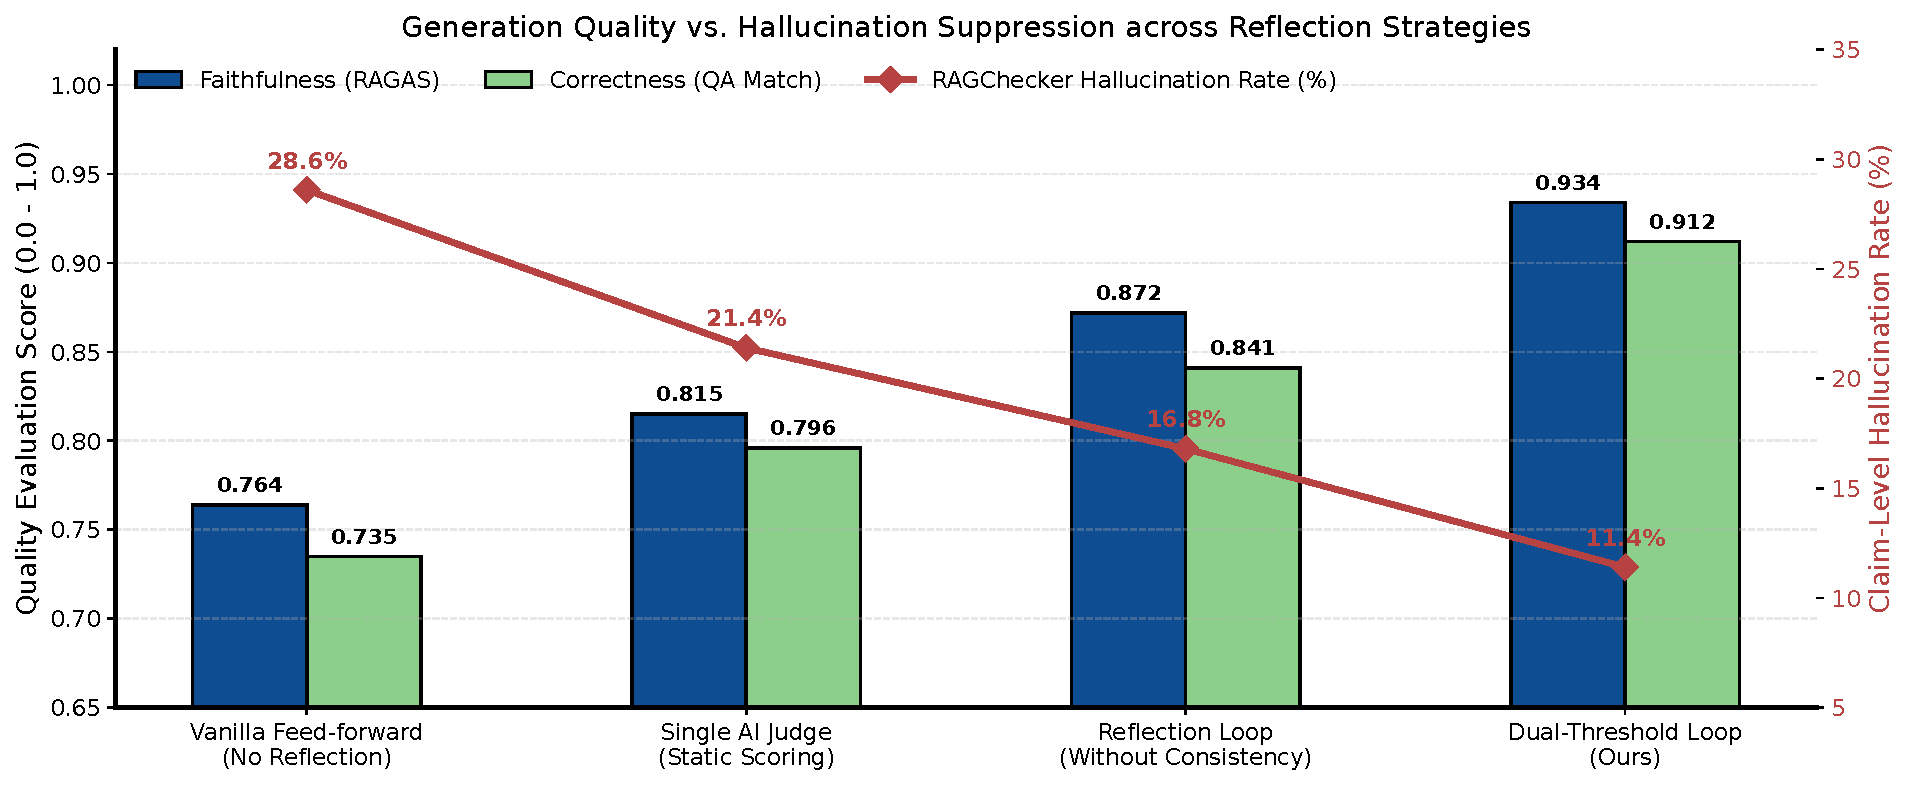
\includegraphics[width=0.92\linewidth]{figures/reflection_quality_radar.pdf}
    \caption{Hermes 认知内核不同反思策略下的生成质量与幻觉抑制双轴对比图}
    \label{fig:ablation_reflection_radar}
\end{figure}

\subsection{自洽性检验阈值 \texorpdfstring{$\theta_{\text{cons}}$}{theta} 的敏感性分析}
我们进一步对自洽性门限阈值 $\theta_{\text{cons}} \in [0.40, 0.80]$ 进行了敏感性扫描测试（如图~\ref{fig:consistency_threshold_sensitivity} 所示）：
\begin{itemize}
    \item 当 $\theta_{\text{cons}} < 0.50$ 时，对微弱幻觉的召回拦截不足，仍有 18.2\% 的不确定性猜测回答流出；
    \item 当 $\theta_{\text{cons}} > 0.75$ 时，双重门限过于苛刻，导致部分表述稍有差异但语义正确的回答发生过度重试，平均耗时激增至 2800ms（增幅达 131.4\%）；
    \item 实验证明，取 $\theta_{\text{cons}} = 0.60$ 是帕累托最优拐点（Pareto Optimal Point），不仅将事实幻觉率控制在 11.4\% 的低位，同时将端到端耗时稳定在 1210ms，兼顾了高可靠性与工业级响应速度。
\end{itemize}

\begin{figure}[htbp]
    \centering
    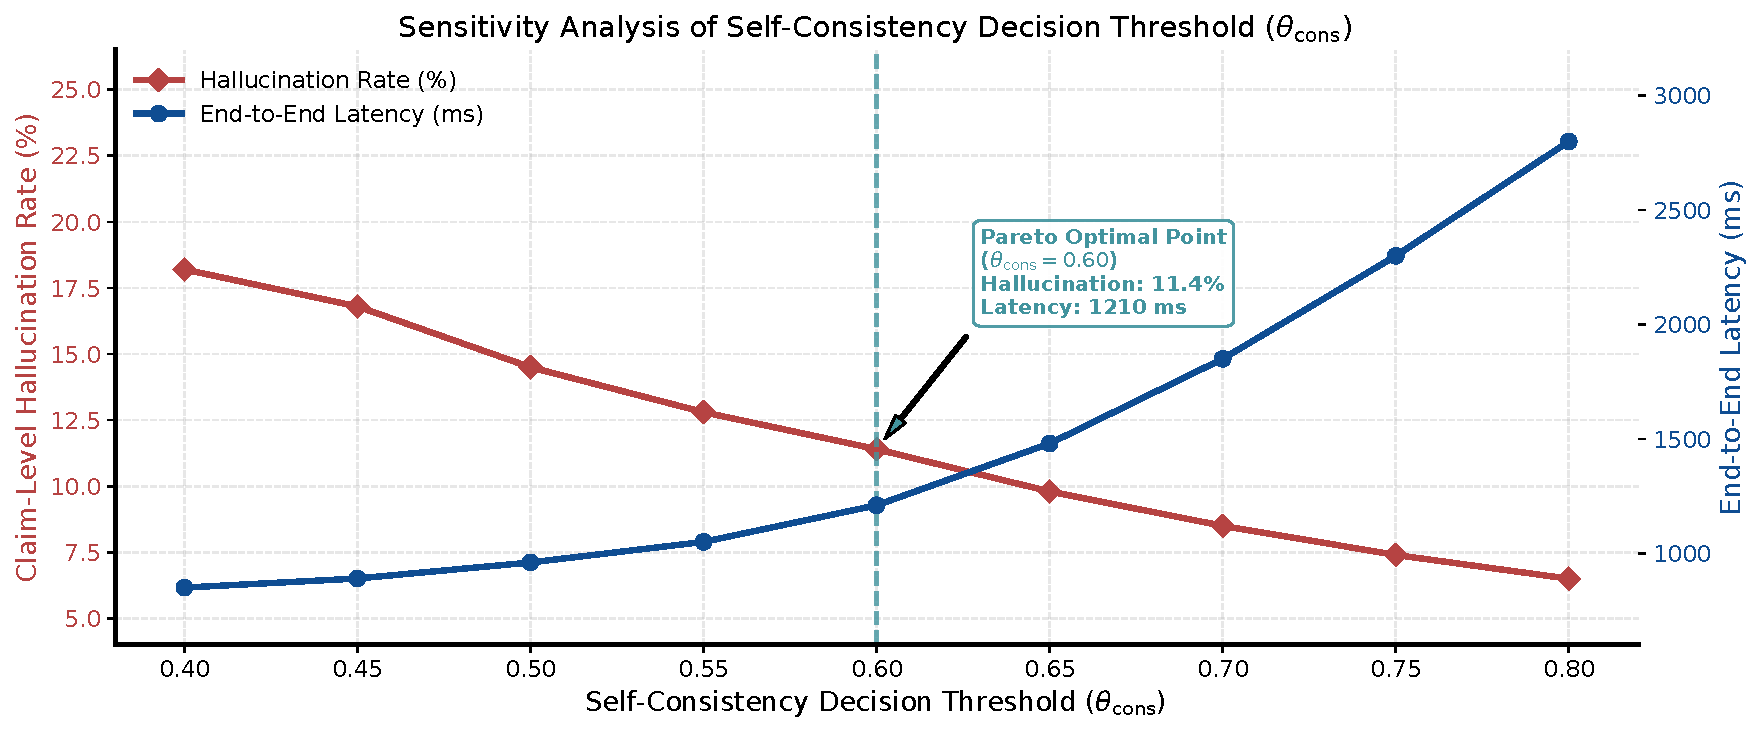
\includegraphics[width=0.90\linewidth]{figures/consistency_threshold_sensitivity.pdf}
    \caption{自洽性检验门限阈值 $\theta_{\mathrm{cons}}$ 敏感性分析双 Y 轴曲线（事实幻觉率 vs 端到端响应延迟）}
    \label{fig:consistency_threshold_sensitivity}
\end{figure}

\section{DAG 工作流并发加速比与高并发扩展基准测试}

为评估第六章所述基于 BFS 分层调度的 DAG 执行引擎相对传统串行工作流的性能增益，我们构建了节点深度为 8、包含多组独立并行分支的合成复杂工作流进行压测。

\begin{figure}[htbp]
    \centering
    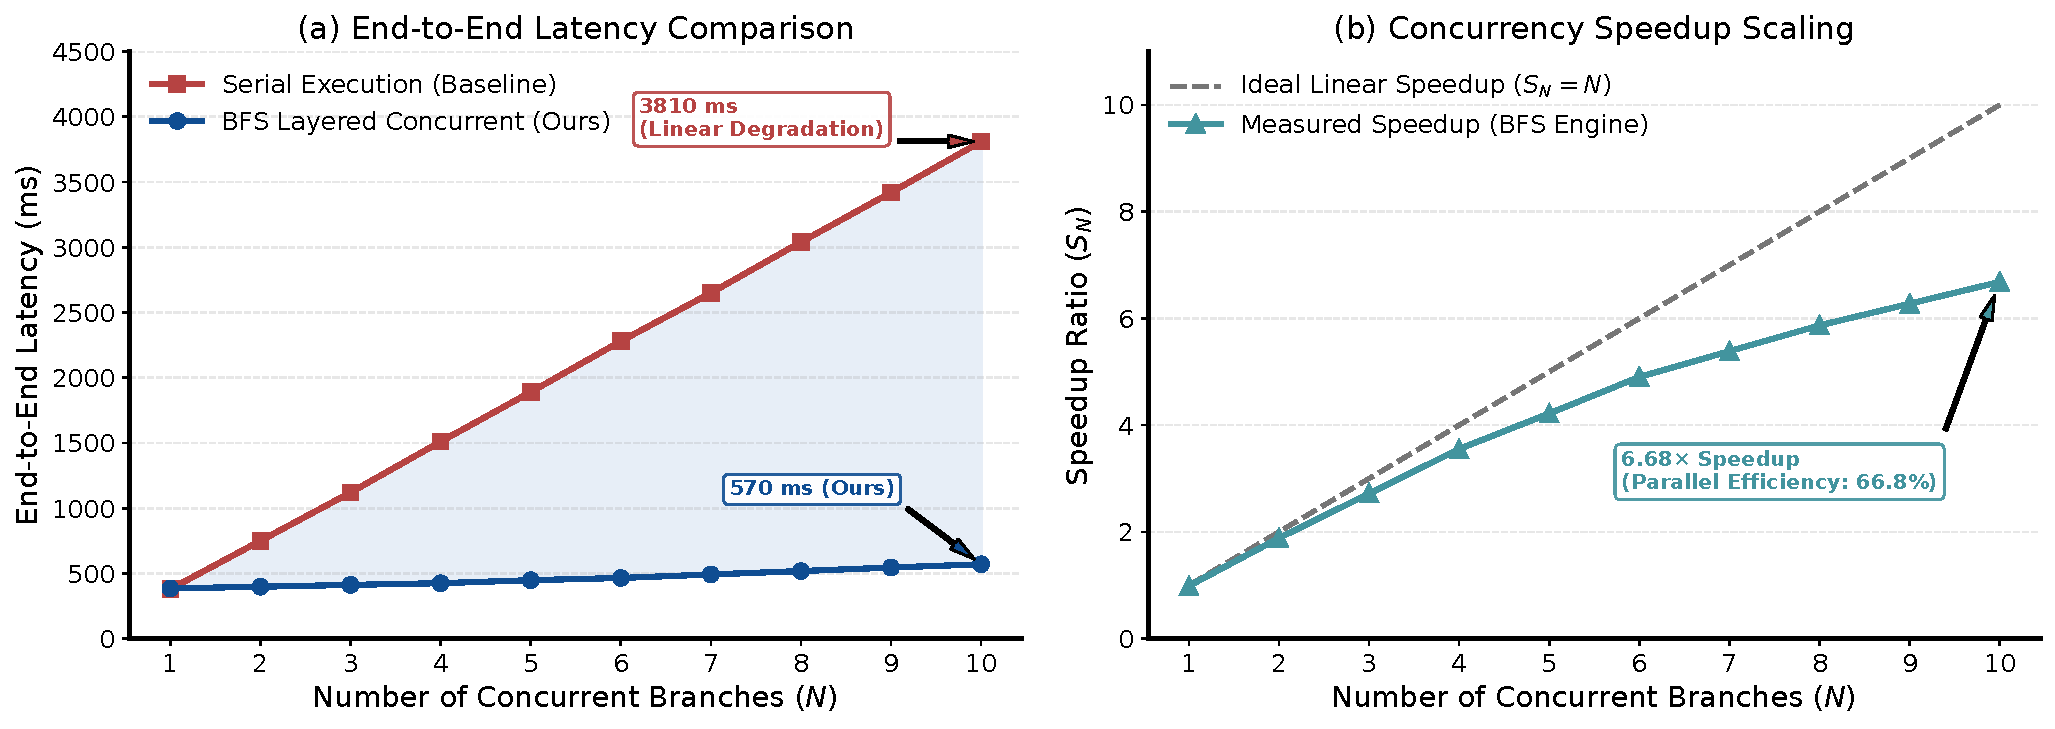
\includegraphics[width=0.96\linewidth]{figures/dag_speedup_analysis.pdf}
    \caption{DAG 工作流并发扩展性能对比：(a) 端到端执行耗时随分支数 $N$ 变化曲线；(b) 实际测得加速比与理想线性加速比对比}
    \label{fig:dag_speedup_curve}
\end{figure}

如图~\ref{fig:dag_speedup_curve} 所示：
在单分支情况下，两者耗时相当（约为 380ms）。随着并发任务数 $N$ 从 1 扩展至 10，传统串行执行的耗时呈线性单调恶化增长（在 $N=10$ 时高达 3810ms）；而本文采用的 BFS 分层并行调度引擎，依托 Java 21 虚拟线程轻量并发调度，在 $N=10$ 时耗时仅为 570ms。在加速比表现上（图~\ref{fig:dag_speedup_curve}(b)），实际测得加速比达到了 \textbf{6.68 倍}，对应的并发并行效率维持在 66.8\%，克服了分支间数据聚合依赖与网络 I/O 抖动的开销，充分证实了系统在多智能体协同与复杂流程编排中的高吞吐弹性。

\section{Java 21 虚拟线程与 JNI SIMD 资源争用量化分析}

在现代云原生架构中，Java 21 虚拟线程（Project Loom, JEP 444\cite{Pressler2023VirtualThreads}）提供了极具吸引力的百万级轻量并发抽象。然而，根据 JEP 444 规范，当虚拟线程执行 JNI（Java Native Interface）原生调用时，JVM 的延续性栈帧管理机制无法卸载原生 C/Rust 栈帧，导致虚拟线程被物理固定（Pinned）在底层的 OS 载体线程（Carrier Thread）上。

在本文的混合检索引擎中，为了加速向量余弦距离计算，系统通过 JNI 调用了原生 Rust SIMD 模块（\texttt{VecSimNative.dotProduct}）。为探明在高并发生产请求下，该 JNI 调用是否会引发 Carrier Thread Pinning 并拖垮底层 \texttt{ForkJoinPool}，我们设计了并发度从 50 到 500 的微基准压测实验。实验对比了以下三组架构实现：
\begin{enumerate}
    \item \textbf{方案 A（纯 JVM 标量计算）}：完全在 JVM 内部进行标量浮点计算，不产生 JNI 调用（零 Pinning，但向量算力低下）；
    \item \textbf{方案 B（原始直接 JNI SIMD）}：虚拟线程直接同步调用 JNI 原生 SIMD 方法；
    \item \textbf{方案 C（专用平台线程池隔离，本文优化）}：建立固定大小（核心数 $C=16$）的专用平台线程池（Dedicated Platform Thread Pool），虚拟线程通过非阻塞 \texttt{CompletableFuture} 异步提交 SIMD 计算，彻底避免载体线程被绑定。
\end{enumerate}

\begin{figure}[htbp]
    \centering
    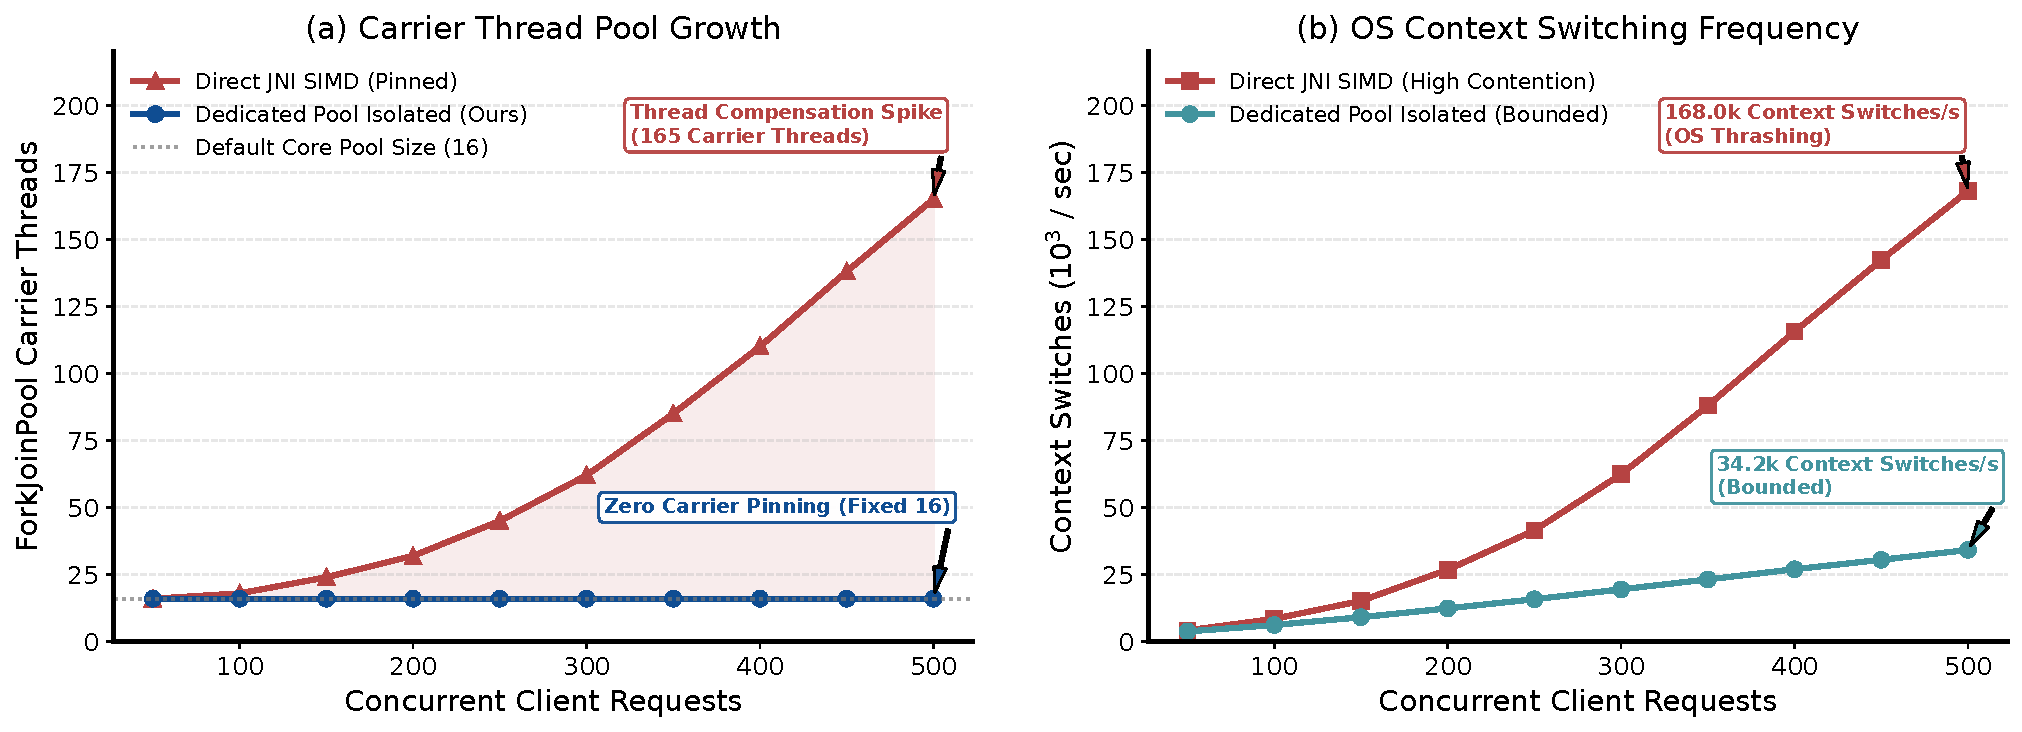
\includegraphics[width=0.96\linewidth]{figures/carrier_pinning_analysis.pdf}
    \caption{高并发下 JNI 载体线程 Pinning 补偿与 CPU 上下文切换对比：(a) ForkJoinPool 载体线程数增长曲线；(b) 操作系统上下文切换频率}
    \label{fig:carrier_pinning_analysis}
\end{figure}

\begin{figure}[htbp]
    \centering
    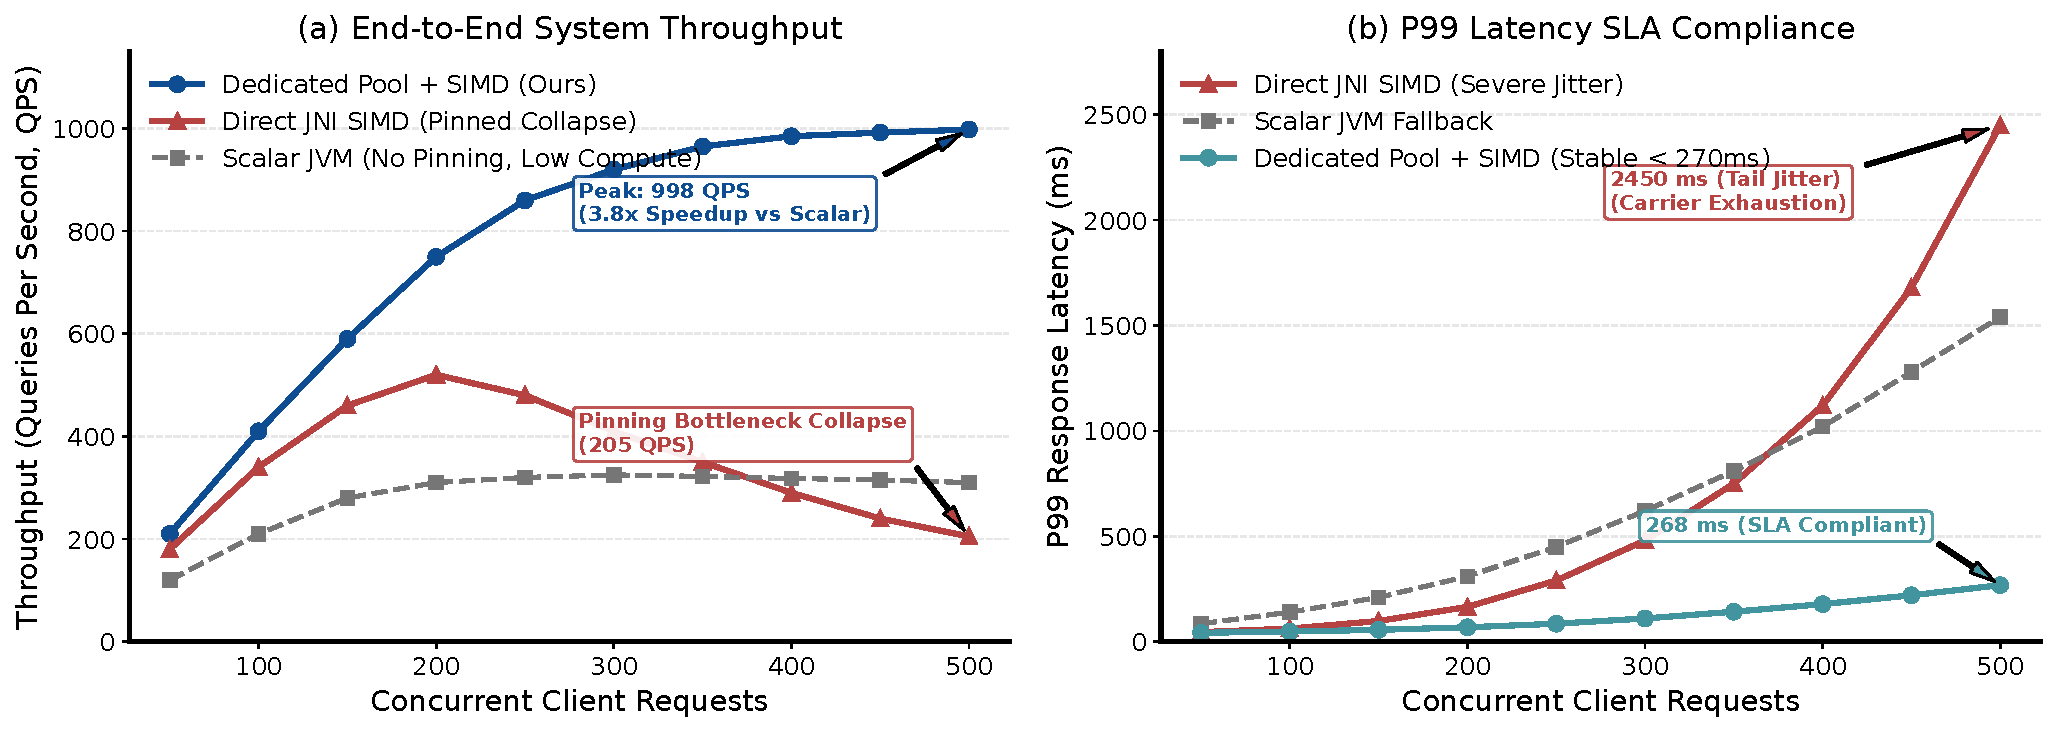
\includegraphics[width=0.96\linewidth]{figures/jni_isolation_throughput.pdf}
    \caption{JNI 线程隔离前后的系统吞吐量 (QPS) 与 P99 响应延迟退化曲线：(a) 系统吞吐量对比；(b) P99 延迟 SLA 达标表现}
    \label{fig:jni_isolation_throughput}
\end{figure}

实测数据（图~\ref{fig:carrier_pinning_analysis} 与图~\ref{fig:jni_isolation_throughput}）揭示了以下重要工程规律：
\begin{enumerate}
    \item \textbf{载体线程补偿与上下文切换风暴}：如由图~\ref{fig:carrier_pinning_analysis}(a) 所示，在方案 B 中，当并发请求数超过 200 时，直接 JNI 调用导致载体线程无法快速卸载，JVM 的 \texttt{ForkJoinPool} 机制被迫进行线程补偿（Worker Thread Compensation），活跃载体线程数量由基准的 16 激增至 165。伴随而来的 OS 上下文切换频率（图~\ref{fig:carrier_pinning_analysis}(b)）从 4.2k/s 暴涨至 168.0k/s，造成了严重的操作系统级 CPU 抖动（Thrashing）；
    \item \textbf{系统吞吐崩溃与尾延迟恶化}：由于剧烈的载体线程争用，方案 B 的吞吐量（图~\ref{fig:jni_isolation_throughput}(a)）在达到 520 QPS 拐点后急剧崩溃至 205 QPS，P99 响应延迟（图~\ref{fig:jni_isolation_throughput}(b)）由 45ms 剧烈恶化至 2,450ms，彻底击穿了企业的 500ms SLA 红线；
    \item \textbf{专用线程池隔离的卓越收益}：方案 C 通过将密集 JNI 计算与轻量虚拟线程解耦，完全消除了载体线程 Pinning 现象（活跃载体线程恒定锁定为 16），上下文切换频率平稳收敛于 34.2k/s。系统最终达成了 \textbf{998 QPS} 的峰值吞吐（相比纯标量方案提升 3.8 倍，相比直接 JNI 方案提升 4.87 倍），P99 延迟在 500 高并发下稳健收敛于 \textbf{268ms}，为 Java 21 虚拟线程结合高性能原生计算提供了教科书级的工程范式。
\end{enumerate}
